\cleardoublepage
\chapter{Introduction}
\label{ch:introduction}
\begin{fullwidth}
  \newthought{In the 6th century B.C.}, Pythagoras discovered that
  dividing a resonating string into simple mathematical ratios
  produced harmonious musical intervals, while arbitrary ratios
  produced dissonance.  His observation is probably the first of the
  many explicit parallels between math and music that have been
  identified since his time. Today, we describe musical pitches as
  integers within a given tuning system. We describe the tuning system
  with a mathematical formula that relates frequency to pitch. Musical
  time, rhythm and meter are commonly described numerically. Musical
  transposition and inversion both mirror mathematical functions and
  borrow their names directly from mathematics.
\end{fullwidth}

As computers, amplifiers, and electronics become our primary tools for
creating manipulating, and performing music, mathematics and music
necessarily become more interconnected. Nearly every modern musical
recording, broadcast, and stream is the summation of many digital
recordings that have been individually discretized, sampled,
mathematically encoded, decoded, and digitally processed numerous
times before ever reaching our ears.\cite{Case2007} It is tempting to
describe music today as applied mathematics, but doing so betrays a
fundamental quality of music: Musicality does not correspond to % come
                                % back to this. replace musicality
                                % with some
mathematical elegance or precision. A musician will diverge from a
musical score to accomplish a particular artistic objective. A
vocalist does not abruptly change a pitch, but gently and carefully
lands on a pitch. A jazz musician might intentionally play slightly
behind the beat. A classical performer knows how to hold a fermata
just long enough. These intentional human artifacts are characterized
more by a feeling than by a formula.

% Because of the computer's inability..., new musical genres have emerged.
The computer's inability to understand feeling has led to new genres
of music like EDM\sidenote[][-25mm]{EDM (Electronic Dance Music)
  features formulaic and repetitive grooves locked to a temporal grid
  and often incorporates aggressive use of digital pitch correction,
  further exaggerating a robotic quality.}, Black
MIDI\sidenote[][-3mm]{Black MIDI is a musical genre that uses low
  fidelity audio samplers with a large number of MIDI notes over a
  short time. A single three minute Black MIDI track is likely to have
  over 100,000 MIDI notes. The name refers to the solid black
  appearance of the piano score.}, and Demoscene\sidenote{Demoscene
  music celebrates digital synthesis of compositionally complex
  electronic music and audio visualizations, using low level software
  interfaces and including the design and programming of the music
  synthesizers as part of the composition.}, but these styles of music
feature (rather than fix) the inhuman nature of computers. If we want
to integrate a computer into the performance or production of truly
expressive music, we must capture perceived feelings formulaically
and program the computer to reproduce them. This thesis describes
three different, but related projects that confront this challenge from
contrasting perspectives: \refmod, \polytempic, and \thesis.

\section{\refmod}
\label{sec:refmod-intro}
\newthought {Music and space} are intimately connected. The first
project, described in \autoref{ch:ref-mod}, explores how we can
compose music using acoustic reflections in architectural space as a
medium. \refmod is a software tool that lets us design and experiment
with abstract acoustic lenses or ``sound mirrors'' in two
dimensions. It is directly inspired by the music and architecture of
Iannis Xenakis, a 20th century composer, music theorist, architect,
and engineer. His collected works provide guidance and perspective to
all the projects in this thesis.

\section{\polytempic}
\label{sec:polytempic-intro}

\newthought{Music and Time} are inseparable. All music flows through
time and depends on temporal constructs - the most common being meter
and tempo. Accelerating or decelerating tempi are common in many
styles of music, as are polyrhythms.  Music with multiple simultaneous
tempi or \textit{polytempic music} is less common, but still many
examples can be found. Fewer examples of music with simultaneous tempi
that shift relative to each other exist, however, and it is difficult
for musicians to accurately perform changing tempi in
parallel. Software is an obvious choice for composing complex and
challenging rhythms such as these, but existing compositional software
makes this difficult. \polytempic offers a solution to this challenge
by describing a strategy for composing music with multiple
simultaneous tempi that accelerate and decelerate relative to each
other. In \autoref{ch:polytempic} we derive an equation for smoothly
ramping tempi to converge and diverge as musical events within a
score, and show how this equation can be used as a stochastic process
to compose previously inaccessible sonorities.

\section{\thesis}
\label{sec:hypercompression-intro}
\newthought{We usually think of compression} in terms of
\emph{reduction}: We use data compression to reduce bit-rates and file
sizes and audio compression to reduce dynamic range. Record labels use
of dynamic range compression as a weapon in the \emph{loudness
  war}\sidenote[][-3cm]{``Loudness War'' is the popular name given to
  the trend of increasing percieved loudness in music recordings.
  Beginning in the 1990s, record labels have attempted to make their
  music louder than the competition, at the expense of audio
  fidelity.}\cite{Deruty2014a}, has resulted in some of today's music
recordings utilizing no more dynamic range than a 1909 Edison
cylinder.\cite{Katz2007} A deeper study of dynamic range compression,
however, reveals more subtle and artistic applications beyond that of
reduction. A skilled audio engineer can apply compression to
improve intelligibility, augment articulation, smooth a performance,
shape transients, extract ambience, de-ess vocals, balance multiple
signals, or even add distortion.\cite{Case2007} At its best, the
compressor is a tool for temporal shaping, rather than a tool for
dynamic reduction.

\thesis expands the traditional model of a dynamic range compressor to
include spatial shaping. While unconventional, spatial processing is a
very natural fit for the compression paradigm. Sound is a medium that
exists in time as well as in space.\sidenote{Converting measurement of
  sound from the cycles per second (in the temporal domain) to
  wavelength (in the spatial domain) is a common objective in
  acoustics and audio engineering practices. See \textit{The Sound
    Reinforcement Handbook} by G. Davis for examples.} The mathematics
and implementation of the Hypercompressor are described in detail in
\autoref{ch:hypercompressor}.

%\paragraph{Performance}
\thesis was used in the live performance of \textit{De
  L'Exp\'{e}rience}, a new musical work by composer Tod Machover for
Narrator, Organ, and Electronics. During the premier at the Maison
Symphonique de Montr\'{e}al in Canada, \thesis was used to blend the
electronics with the organ and the acoustic space. 
A detailed description of how \thesis featured in this performance is
also discussed in \autoref{ch:hypercompressor}.

\section{Background}
\label{sec:background}
These projects build on the work and ideas of Iannis Xenakis, a 20th
century composer, architect, and engineer. Xenakis spent his youth
reading about astronomy, archeology, ancient literature, and
mathematics.\cite[]{Hoffmann2015} He studied music and engineering at
the Polytechnic Institute in Athens, Greece. By 1948, Xenakis had
graduated from the university and moved to France where he began
working for the French architect, Le Corbusier. The job put his
engineering skills to use, but Xenakis also wanted to continue
studying and writing music. While searching for a music mentor, he
approached Oliver Messiaen\sidenote{Messiaen was a prolific French
  composer known for rhythmic complexity. He was also regarded as a
  fantastic music teacher, and his students include Karlheinz
  Stockhausen, Pierre Boulez, and Quincy Jones.}, and asked for advice
on whether he should study harmony or counterpoint. Messiaen later
described his conversation with Xenakis:
\begin{quotation}``I think one should study harmony and
  counterpoint. But this was a man so much out of the ordinary that I
  said: No, you are almost 30, you have the good fortune of being
  Greek, of being an architect and having studied special
  mathematics. Take advantage of these things. Do them in your
  music.''\cite{Service2013}
\end{quotation}
In essence, Messiaen was rejecting Xenakis as a student, but we can
see how Xenakis ultimately drew from his disparate skills in his
compositions. The score for his 1945 composition \textit{Metastasis}
(figure~\ref{fig:metastasis}) resembles an architectural blueprint as
much as it does a musical score.

\begin{figure*}[h]
  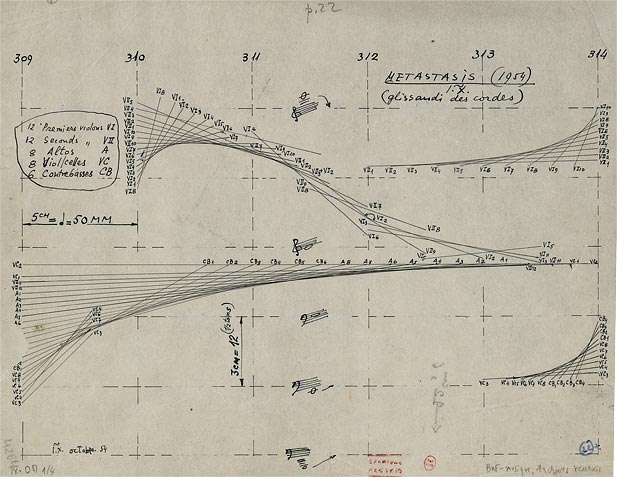
\includegraphics[width=\linewidth]{XenakisMetastasis.jpg}
  \caption{Excerpt from Iannis Xenakis' composition,
    \textit{Metastasis} (1954), measures 309-314. This score in this
    image was then transcribed to sheet music for the orchestral
    performance.}
  \label{fig:metastasis}
\end{figure*}

\subsection{The Philips Pavilion}
\label{sec:philips-pavilion-1}
\begin{figure}[h]
  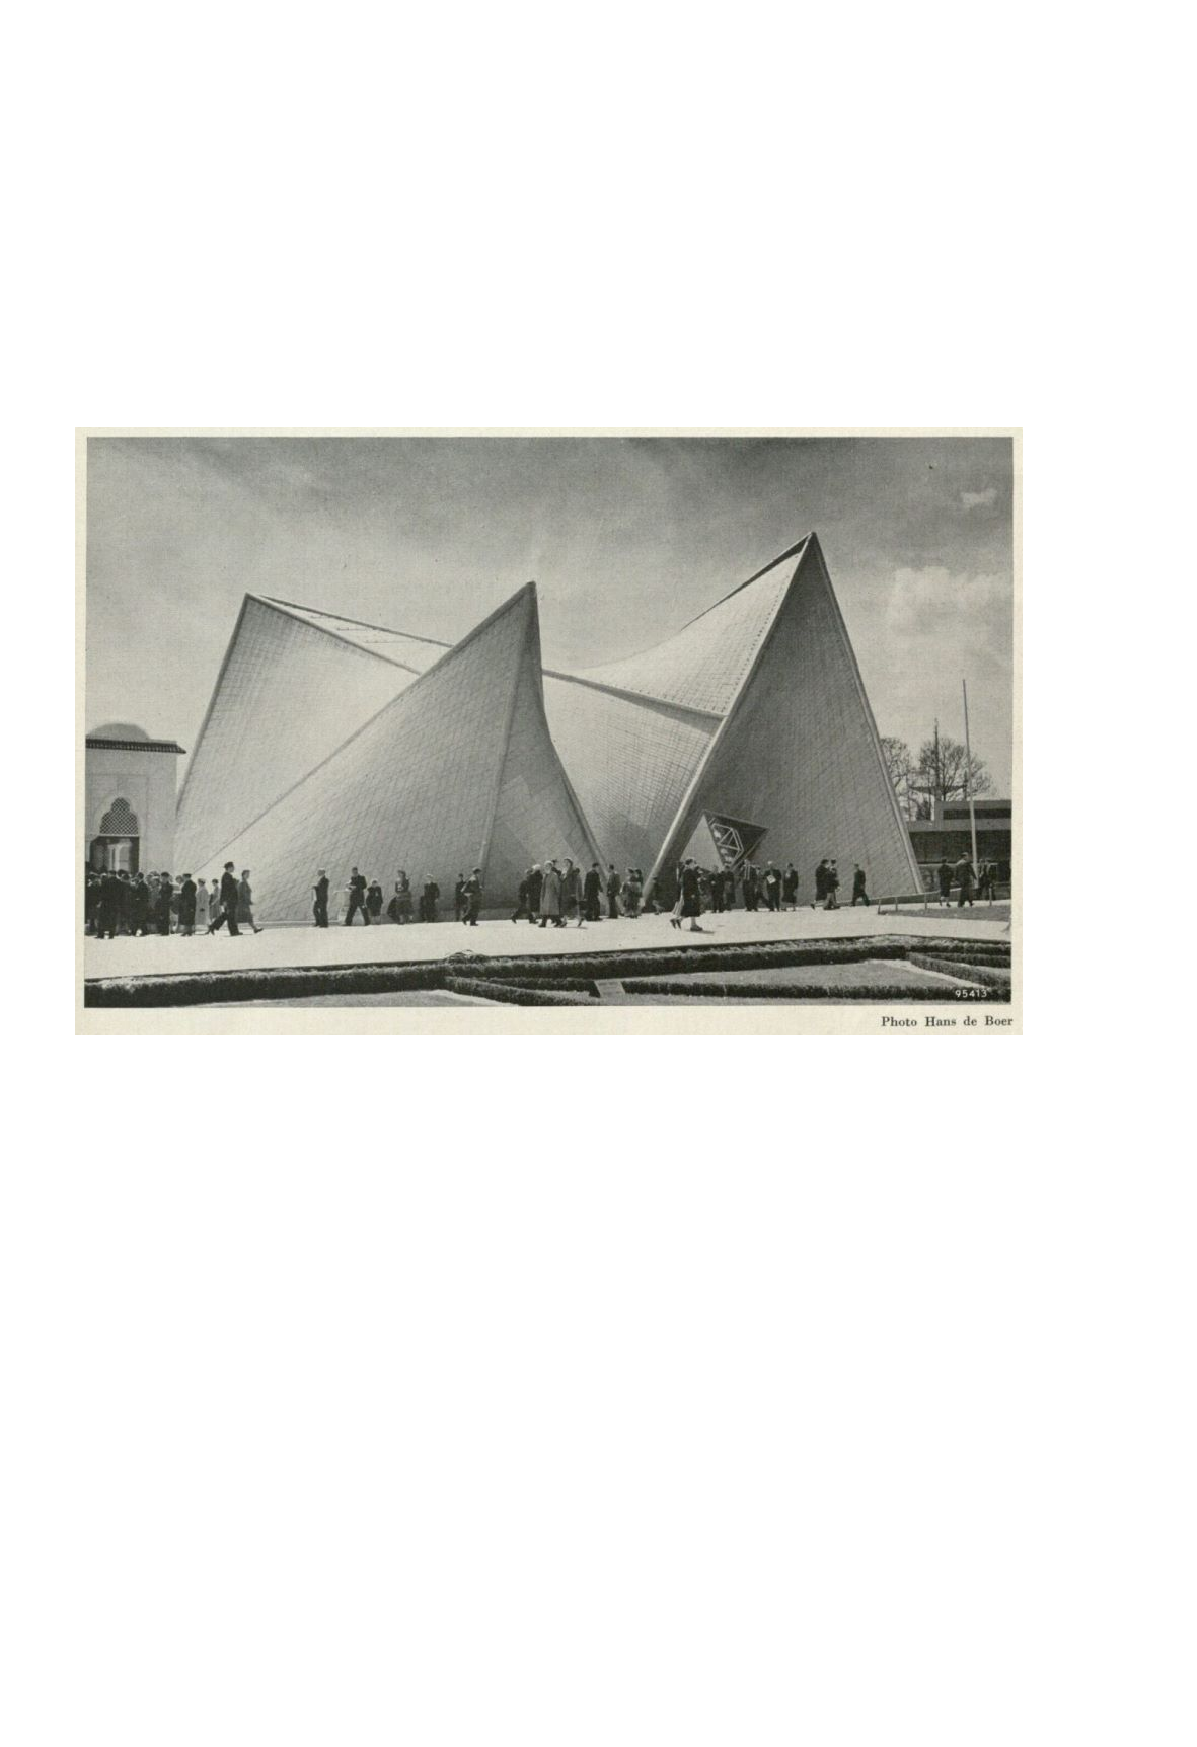
\includegraphics[width=\linewidth]{PhilipsPavilion-TechnicalReview-00.pdf}
  \caption{The Philips Pavilion at the 1958 Brussels World Fair as
    shown in Volume 20 of the \textit{Philips Technical Review}, 1959.}
  \label{fig:philips-pavilion-photo}
\end{figure}
In 1956, Le Corbusier was approached by Louis Kalff (Artistic Director
for the Philips corporation) and asked to build a pavilion for the
1958 World's Fair in Brussels. The pavilion was to showcase the sound
and lighting potential of Philips' technologies. Le Corbusier
immediately accepted, saying:
\begin{quotation}
  ``I will not make a pavilion for you but an Electronic Poem and a
  vessel containing the poem; light, color image, rhythm and sound
  joined together in an organic synthesis.''\cite{Lopez2011} 
\end{quotation}
The final product lived up to Le Corbusier's initial description. It
included:\cite{Lombardo2009}
\begin{enumerate}
\item A concrete pavilion, designed by architect and composer Iannis
  Xenakis
\item \textit{Interlude Sonoire} (later renamed \textit{Concret PH}), a
  tape music composition by Iannis Xenakis, approximately 2 minutes
  long, played between performances, while one audience left the
  pavilion and the next audience arrived
\item \textit{Po\`{e}me \'{E}lectronique}, a three channel, 8 minute
  tape music composition by composer Edgard Var\`{e}se
\item A system for spatialized audio across more than 350 loudspeakers
  distributed throughout the pavilion
\item An assortment of colored lighting effects, designed by Le Corbusier in
  collaboration with Philips' art director, Louis Kalff
\item Video consisting mostly of black and white still images,
  projected on two walls inside the pavilion
\item A system for synchronizing playback of audio and video,
  with light effects and audio spatialization throughout the
  experience
\end{enumerate} 

\paragraph{Role of Iannis Xenakis} During the initial design stage, Le
Corbusier decided that the shape of the pavilion should resemble a
stomach, with the audience entering through one entrance and exiting
out another. He completed initial sketches of the pavilion layout and
then delegated the remainder of the design to
Xenakis.\cite{Clarke2012}

The architectural evolution of the pavilion from Le Corbusier's early
designs (figure~\ref{fig:le-corbusier-sketch}) to Xenakis' iterations
(figure~\ref{fig:xenakis-draw}), illustrates the profound impact that
Xenakis had on the project. An article in the \textit{Philips
  Technical Review}\cite{philips1958} gives a wonderfully detailed
account of Xenakis' process in restructuring the design:\sidenote{\TODO{Clean this section.}}
\begin{enumerate}
\item Xenakis was aware that parallel walls and concave spherical
  walls would both negatively impact audio perceptibility due to repeated
  or localized acoustic reflections.
\item To accommodate musical purpose of the space he decided to
  explore surfaces with varying curvature...
\item 
  \begin{marginfigure}
    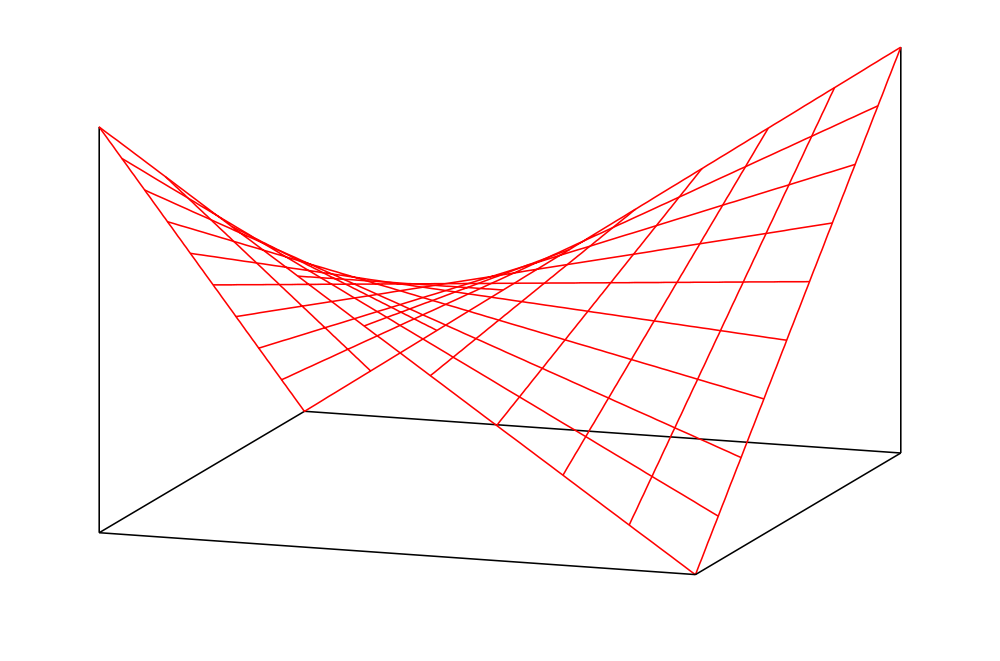
\includegraphics{hyperbolic-paraboloid}
    \caption{A ruled surface. For a surface to be considered ``ruled''
      every point on the surface must be on a straight line, and that
      line must lie on the surface. In Xenakis' time, ruled surfaces
      were useful in architecture, because they simplified the
      construction of curved surfaces by using straight beams.}
    \label{fig:ruled-surface}
  \end{marginfigure}...leading him to consider ruled surfaces such as
  the conoid and hyperbolic paraboloid. 
\end{enumerate}
Through this process, we see Xenakis utilizing the skills that he
learned at the Polytechnic Institute and continued to develop while
working with Le Corbusier. He also understood the mathematical
formation of the ruled surfaces that make up the structure. These
surfaces even look familiar to the Metastasis score
(figure~\ref{fig:metastasis}). In his 1963 book, \textit{Formalized
  Music}, Xenakis explicitly states that the Philips Pavilion was
inspired by his work on \textit{Metastasis}.

\begin{figure*}[]
  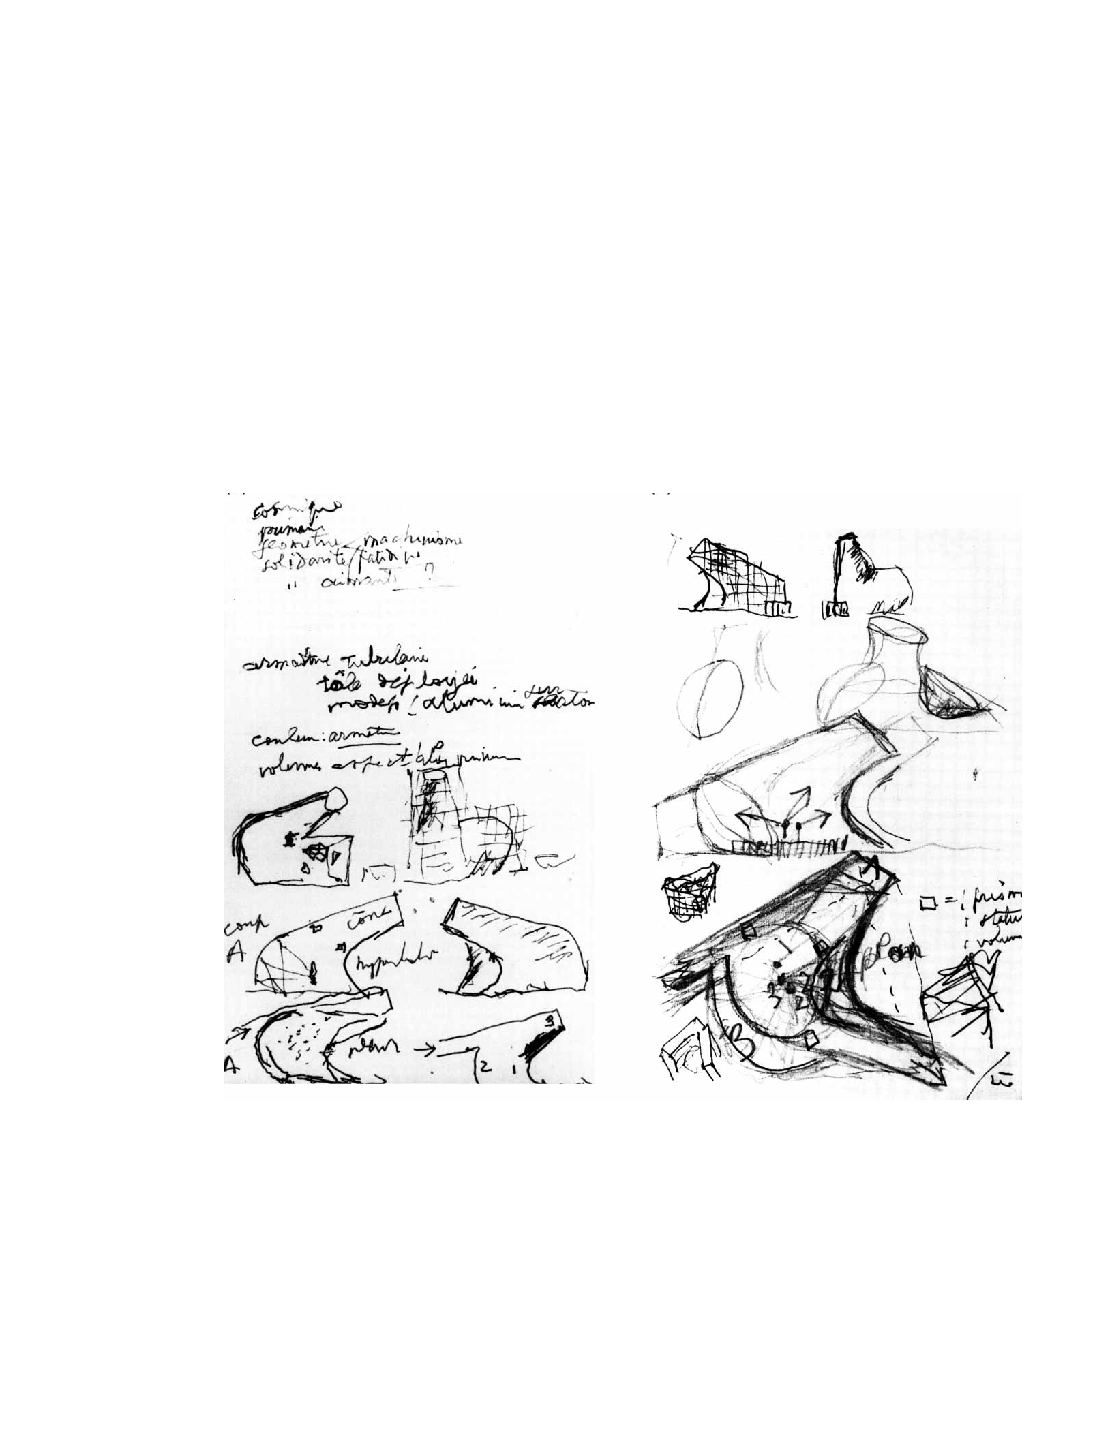
\includegraphics[width=\linewidth]{LeCorbusierDraw.pdf}
  \caption{Le Corbusier's design sketches for the Philips Pavilion,
    September \textendash{} October, 1956 (\textcircled{c} 2012
    Artists Rights Society, New York/ADAGP, Paris/FLC)}
  \label{fig:le-corbusier-sketch}
\end{figure*}

\begin{figure*}[h]
  % XenakisSketch.pdf or PhilipsDrawings.jpg
  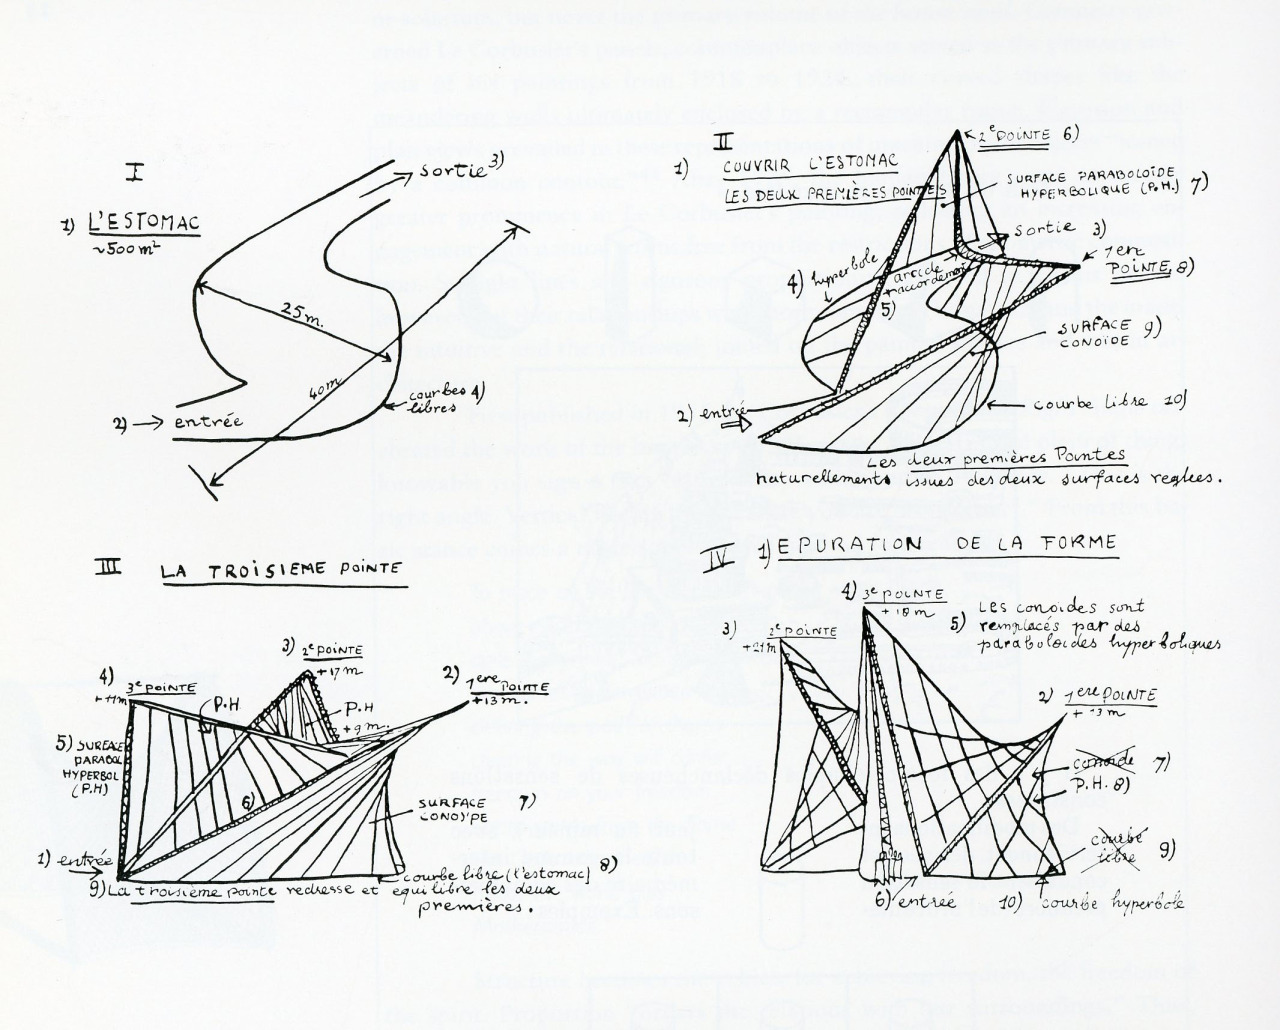
\includegraphics[]{PhilipsDrawings.jpg}
  \caption{Xenakis' early drawings of the Philips Pavilion as
    documented in volume 20 of the \textit{Philips Technical Review}.}
  \label{fig:xenakis-draw}
\end{figure*}

\section{Architecture and Music in Space and Time}
\label{sec:introduction-conclusion}

In \textit{Formalized Music}\cite{xenakis1992formalized}, Xenakis
describes how developments in music theory mimic equivalent
developments in philosophy, mathematics, and the sciences. Plato, for
example, believed that all events transpire as determined by cause and
effect. While Plato and Aristotle both described causality in their
writing, it was not until the 17th century that controlled experiments
and mathematics corroborated the theory.\sidenote{In 1687, Isaac
  Newton published \textit{Philosophi\ae{} Naturalis Principia
    Mathematica} (\textit{Mathematical Principles of Natural
    Philosophy}), in which he compiled the 3 laws of motion that set
  the foundation for the study of \emph{classical mechanics}.}
Similarly, music theory has historically employed causal rules to
describe counterpoint, tonality, and harmonic movement.\sidenote{\TODO{Add example}}

Causality was largely used to describe physical phenomena until the
19th century when statistical theories in physics began to include
probabilistic notions.\sidenote{The Maxwell-Boltzmann distribution,
  which was first derived by James Clerk Maxwell in 1860, describes
  the probability distribution for the speed of a particle within an
  idealized gas. For more see
  \url{http://plato.stanford.edu/entries/statphys-statmech/}} Xenakis
noticed that more contemporary fields like \emph{probability theory}
generalize and expand on the antecedent theories of causality. Xenakis
thought that music composition should naturally follow the progression
that physics did, with music theory generalizing and expanding on
causal rules that had existed previously. Indeed, starting in the late
19th century and early 20th century, composers like Strauss and
Debussy began to bend the existing rules of music theory, composing
music that branched away from the causal and tonal theories of the
time. With the rise of serialism\sidenote{Serialism is a technique for
  musical composition in which instances of musical elements (such as
  pitch, dynamics, or rhythm), are given numerical values. Sequences
  built from the values are ordered, repeated and manipulated
  throughout the composition.}  and indeterminate music\sidenote{In
  music, indeterminacy refers to the use of chance (such as rolling
  dice or flipping coins) as part of the compositional process.},
composers such as Stockhausen, Boulez, John Cage, Aaron Copland, and
B\'{e}la Bart\'{o}k began to use probability and chance in
composition, the same way that physicists were using probability to
describe the material world. 

To Xenakis' mind, serial music was no less causal than the music it
intended to supersede. He described serial music as embodying
``virtually absolute determinism.''\cite{xenakis1992formalized}
Xenakis saw music theory as a sub-set of mathematics and algebra:
While musicians have a different vocabulary, they also use
mathematical principles to describe and compose music. Because Xenakis
understood mathematics as well as music, he was able to identify how
even in serialism and indeterminate music, composers were only
utilizing a small subset of algebraic theory. In his own music,
Xenakis wanted to generalize and expand the causal framework that
musicians and theorists had been using to compose and understand
music, paralleling similar developments in physics and
mathematics. As a reference to \emph{chance}, or \emph{stochos},
Xenakis coined the term \emph{stochastic music} to describe his
development.\sidenote{\TODO{Clarify}}

Xenakis' book, \textit{Formalized Music} gives a verbose explanation
of stochastic music. Some authors have interpreted his description
more explicitly. In \textit{Audible Design}, Trevor Wishart describes
the stochastic process used to compose stochastic music as:
\begin{quotation}
  ``A process in which the probabilities of proceeding from one state,
  or set of states, to another, is defined. The temporal evolution of
  the process is therefore governed by a kind of weighted randomness,
  which can be chosen to give anything from an entirely determined
  outcome, to an entirely unpredictable one.''\cite{Wishart1994}
\end{quotation}
% It could be that the lack of a single clear definition by Xenakis is
% the reason that few composers today identify their work as stochastic
% music.

\paragraph{Xenakis' Reflection} In the Spring of 1976, while defending
his doctoral thesis at the University of Paris, Xenakis emphasized the
relevance of seemingly unrelated disciplines to the creative process. A
translation of his defense includes this statement:
\begin{quotation}
  ``The artist-conceptor will have to be knowledgeable and inventive
  in such varied domains as mathematics, logic, physics, chemistry,
  biology, genetics, paleontology (for the evolution of forms), the
  human sciences, and history; in short, a sort of
  \emph{universality}, but one based upon, guided by and oriented
  toward forms and architectures.''\cite{russolo1986art}
\end{quotation}
From Xenakis' drawings we can deduce that he used the same tools,
skills, and philosophy to imagine and conceive both music and
architecture. His approach elevated both forms and blurred the distinction
between the two. Perhaps if we had kept using pen and paper to design
buildings and write music, the reality today would be closer to the
ideal that he imagined. 

As the ideas that inspired Xenakis and other progressive 20th century
composers were taking root in contemporary music, the culture of
artistic form and composition was already beginning the transition
into the digital domain. There is no reason why digital tools cannot
favor stochastic processes to linearity; there is no reason why
digital tools cannot treat music and architecture as equals. However,
even today, software for composing music still favors static pitches
to glissandi; software for architectural design still favors corners
to curves. Most importantly, the software skills that we use to design
and manipulate space, and the skills that we use to compose music,
mutually exclude each other.

This is where the projects described here make a contribution.  By
drawing from music, mathematics, computer science, acoustics, audio
engineering and mixing, sound reinforcement, multimedia production,
and live performance, we can create tools that allow us to
indiscriminately compose with space and sound.

\section{Universality}
\label{sec:universality}
At the MIT Media Lab, we celebrate the study and practice of projects
that exist outside of established academic disciplines. The Media Lab
(and the media) have described this approach as interdisciplinary,
cross-disciplinary, anti-disciplinary, or post-disciplinary; rejecting
the clich\'{e} that academics must narrowly focus their studies
learning \textit{more and more about less and less}, and eventually
knowing \textit{everything about nothing}.  The projects described
here uphold the vision of both Xenakis and the Media Lab. Each chapter
documents the movitaions and implementation of a new tool for
manipulating space and sound. Each project draws from an assortment of
fields including music, mathematics, computer science, acoustics,
audio engineering and mixing, sound reinforcement, multimedia
production, and live performance. 

% How can we describe and document a project with such broad subject
% material? Within a single discipline, there is an accepted hierarchy
% of concepts, and we are expected to develop a \emph{deep}
% understanding that penetrates this hierarchy. We expect students to be
% literate in algebra, geometry and calculus before studying
% physics. When we describe a physics problem, we depend on an
% established collection of language, notation, and theory.

% This example reveals the curious tension between breadth and depth:
% The \textit{depth} of a disciplinary approach provides the language
% and abstraction that enable us to describe content and communicate at
% a high level. Depth is essential for solving non-trivial
% problems. However, solutions to the most complex and interesting
% real-world projects always span multiple disciplines. It appears we
% need breadth \emph{and} depth simultaneously. The impact of Iannis
% Xenakis and the success of the Philips Pavilion illustrate the
% efficacy of this approach. 

% \TODO{this thesis is an experiment in breadth and depth}

% One of the goals of this thesis is to
% bridge disciplines by describing the material in a way that is
% accessible to readers that are not experts in all the fields
% involved.


%%% Local Variables:
%%% mode: latex
%%% TeX-master: "CharlesHolbrow_MAS_Thesis"
%%% End:
